%\vspace{-0.1in}
\section{Challenges}
\label{sec:challenges}

\subsection{Work with existing routing protocols and hardware}
\label{sec:incremental} Data center routing protocols have to satisfy a variety
of complex requirements regarding fault tolerance, and
security~\cite{beckett2016don}. Operators also invest heavily in  tools and
technologies to monitor and maintain their networks; and these tools are
tailored for the routing protocols that are already deployed.  Thus, operators
are unwilling to deploy a brand-new routing
protocols like~\cite{dally,duato93,dally93,sancho2004,flich2012survey,lash,wu2003fault,glass,duato2001,domke2011,puente1999,dfedst16}
or hardware just for deadlock avoidance --  especially when RoCEv2 (encapsulated in standard UDP packets)
itself can be deployed without any changes to routing.

%itself can be deployed without any changes to routing!
%\footnote{RoCEv2 packets are encapsulated in standard UDP packets.}!

\yibo{However, the widely-used routing protocols, like BGP and OSPF, never attempt to
avoid CBD since they are designed for lossy networks. Moreover, modifying these
protocols to avoid CBD is not trivial.
They are inherently asynchronous distributed systems -- there is no guarantee that all routers will
react to network dynamics (\S\ref{sec:reroute}) at the exact same time. This unavoidably creates transient 
routing loops or CBDs, enough for lossless traffic to create deadlocks. In such cases, 
we cannot ensure both losslessness and deadlock-freedom.

In this paper, instead of making drastic changes to routing protocols, we
explore a different design tradeoff.  Our system, \sysname{}, works with any
unmodified routing protocols and guarantees deadlock-freedom by giving up
losslessness only in certain rare cases. We favor this approach
because it is more practical to deploy, and has negligible performance penalty.}

%Our prerequisite that our design needs to be deadlock-free and that it needs to work 
%with all existing routing, including all the widely used protocols, e.g., BGP and OSPF poses technical challenge. 
%Switches running distributed routing protocols need to react failures locally, hence routing loops and CBDs are 
%unavoidable. Therefore distributed routing, deadlock-free, lossless cannot coexist at the same time.}
%\textcolor{blue}{In this paper, we show how \sysname{} uses multiple lossless queues to avoid deadlock, and once deadlock and lossless are in conflict, we put conflicting packets into lossy queues. In \S~\ref{subsec:exp_performanceoverhead}, we will show that using two lossless queues achieves lossless practically.}

\subsection{Data center networks are dynamic}\label{sec:reroute}

Given that we aim to work with existing routing infrastructures, we must
address the issue that most routing schemes are dynamic -- paths change in
response to link failures or other events.

Figure~\ref{fig:basic_clos} shows a simplified (and small) version
of network deployed in our data center, with commonly used up-down routing (also
called valley-free~\cite{qiu2007toward}) scheme.  In up-down routing, a packet first
goes UP from the source server to one of the common ancestor switches of the
source and destination servers, then it goes DOWN from the common ancestor to
the destination server.  In UP-DOWN routing, the following property holds: when
the packet is on its way UP, it should not go DOWN; when it is on its way DOWN,
it should not go UP. Thus, in {\em normal cases}, there can be no CBD and hence
no deadlock.

However, packets can deviate from the UP-DOWN paths due to many reasons,
including link failures, port flaps etc., which are quite common in data
center networks~\cite{netpilot,f10}. When the up-down property is violated,
packets ``bouncing'' between layers can cause
deadlocks~\cite{shpiner2016unlocking}. See
Figure~\ref{fig:clos_1_bounce}.

In our data centers, we see hundreds of violations of up-down routing per
day. Such routes can persist for minutes or even longer. %Overall, we estimate that $0.001\%$ of the traffic is routed over such paths. This may sound tiny, but given that our network carries exabytes of traffic per day,
The absolute volume of traffic affected by such routing is in tens of terabytes. This makes the threat of deadlocks, as discussed
in~\cite{rdmaatscale,shpiner2016unlocking,hu2016deadlocks} quite real.

\begin{figure}[t]
		\centering
		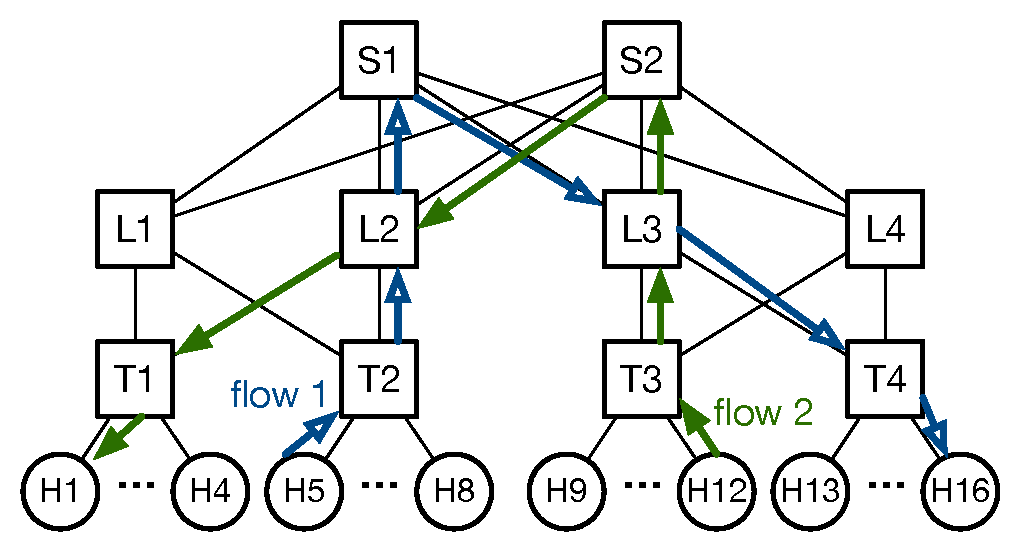
\includegraphics[width=0.38\textwidth] {figs/updown_paths}
		\vspace{-1em}
		\caption{Clos topology with two up-down flows.}
		\vspace{-1.5em}
		\label{fig:basic_clos}
\end{figure}

\subsection{Limited number of lossless queues}
\label{subsec:pfcheadroom}

One idea to solve deadlock is to assign dynamic priority to packets. The
priority of a packet increases as the packet approaches its destination
~\cite{karol2003prevention}.  Such a design requires as many priorities as the largest
path length in the network. 
\jitu{However, there are two practical problems. First,
given the network dynamics, 
the largest path length may not be all that small
(\S\ref{sec:reroute}). Second, the PFC standard
supports only 8 priorities. Worse yet, commodity switches can realistically support only two or three lossless
priorities~\cite{rdmaatscale}.  The problem is that  to
guarantee losslessness, a switch needs to reserve certain amount of
{\it headroom} for absorbing the packets in flight during the time
it takes for the PAUSE message to take effect.


The switch buffers are made of extremely fast and hence extremely expensive
memory, so their size is not expected to increase rapidly even as link speeds
and port counts go up. Some of this buffer must also be set aside to serve lossy
traffic (i.e. normal TCP traffic), which still constitutes a majority of traffic
in data centers.  At the same time, the PFC response time is subject to physical
limits and cannot be arbitrarily reduced.  Thus, even newest switching ASICs are
not expected to support more than four lossless queues.  Hence the solutions
that require a large number of lossless queues are not practical. }


%per port, per lossless queue.
%The headroom is needed to 
%The headroom size depends on many factors, including length
%of cables. See Appendix \ref{APPHEADROOM} for details.  
%, a 32-port 40GbE Ethernet switch needs to reserve 2.76MB of headroom to support one
%lossless queue on all ports. A commodity switch like this typically has
%12MB total buffer\footnote{The memory used to build switch buffers needs to be
%extremely fast (e.g. 32x40GB switch needs memory that can support read/write
%speeds of 1.28 Tbps), and hence is very expensive.}, so 23\%
%of the total switch buffer is needed to support just one lossless priority.

%While this headroom is sufficient to avoid packet drops, in practice, we use a
%slightly larger value to avoid buffer under-flow when the receiver un-pauses the
%sender.  Furthermore, we need to reserve buffers for non-RDMA (i.e. lossy)
%traffic, which is still the dominating traffic in data centers. With these
%constrains, the current commodity switches can typically support just two or
%three lossless classes~\cite{rdmaatscale}.

%New switching ASICs may be able to support more lossless queues by adding more
%memory, using smaller cell size (64-byte) and by reducing the pause frame
%response time. But even these are not expected to support more than four or five
%lossless queues. Hence the solutions that require a large number of lossless
%queues are not practical.

%We now describe how \sysname{} addresses these challenges.
